\chapter{Design of the Qubit Characteristic}
\section{Circuit design}
We designed the circuit depicted in figure \ref{fig:transmission_line_qubit} so that the resonance frequency of the resonator $f_r$ sweeps the range from 6GHz to 11GHz with 250MHz steps: to do so we used the analitical formula for the resonance frequency and found the values of $Lr1$ for each frequency. The two edges values of $Lr1$ are $14.072nH$ and $4.187nH$ for $f_r=6GHz$ and $f_r=11GHz$ respectively. Concerning the Qubit, we calculated the value of $Lq1$ to be $23.45nH$ to have a resonance frequency of $f_q=6GHz$, while the value of $Rq1$ is set to $8.841M\Omega$ to have a quality factor of $Q=10^{4}$. 
\section{Analysis of the simulation}
\begin{figure}[h]
\centering
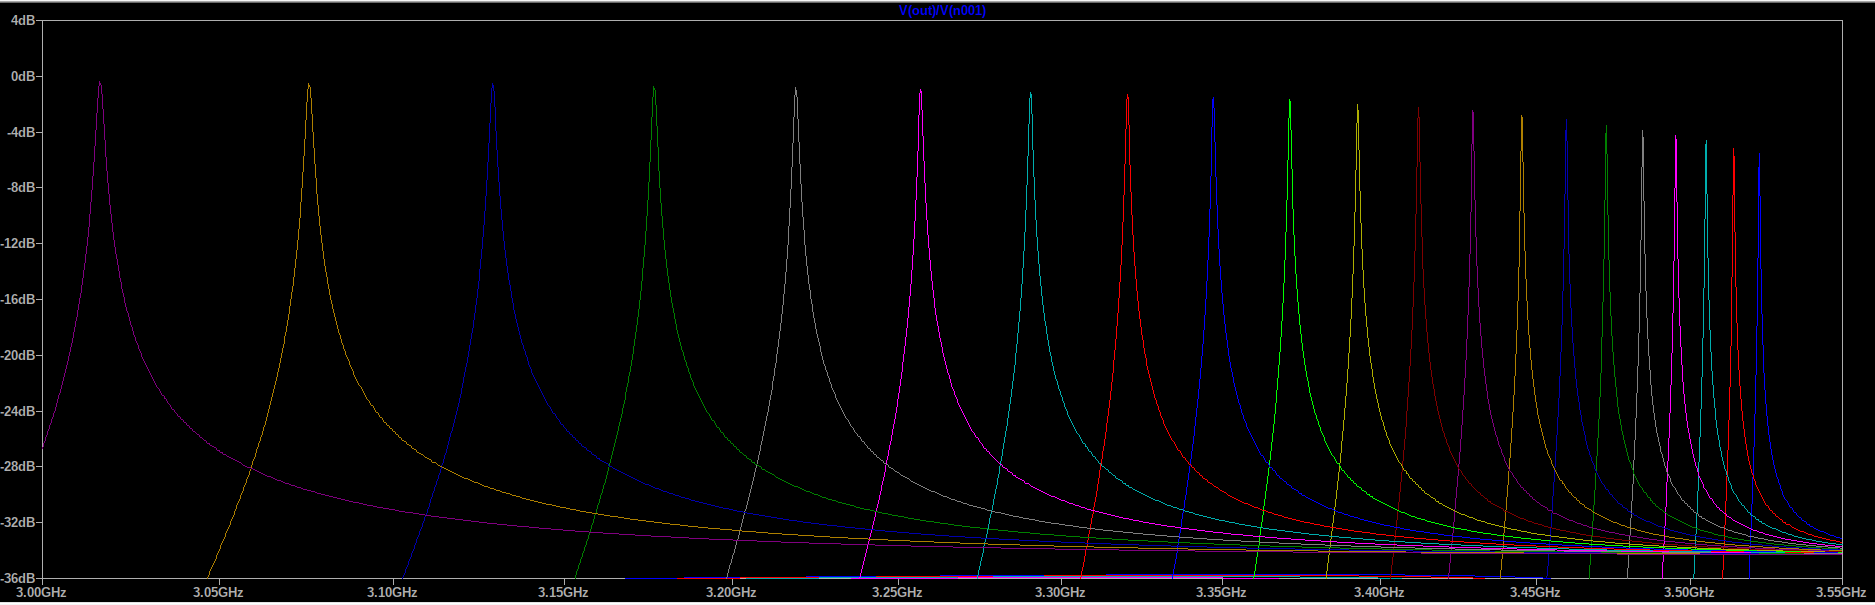
\includegraphics[width=0.8\linewidth]{exercise 6/graph_7_bigg.png}
\caption{Transfer function with given parameters.}
\label{fig:graph}
\end{figure}
The Bode diagram in figure \ref{fig:graph} shows the tranfer function $S=\frac{V_{out}}{V_{in}}$ where $V_{out}$ is the voltage across $R2$ and $V_{in}$ is the voltage across $R1$.
The different resonance frequencies obtained correspond to the different values of $Lr1$ and so to the different values of $f_r$. 
\subsection{Coupled Regime}
When $f_r$ is tuned close to the qubit frequency $f_q$ ($\Delta = f_r - f_q \approx 0$), the system enters the strong coupling regime. In this situation, that corresponds to the resonance observed at $\approx3.01$GHz in the diagram, the qubit and the resonator undergo \textbf{hybridization}. Here, we observe a lower quality factor of the system (the peak has a wider bandwidth) due to the fact that the resonator and the qubit are strongly coupled, and the energy can be efficiently exchanged between them, resulting in a dissipation of energy through the resistance $Rq1$, causing the system to deviate from the high-Q characteristics of an uncoupled, ideal resonator. However, in such lower frequencies, the impedance of $Cg$ is higher, so the input signal is less affected by the dissipative element of the qubit, resulting in a higher gain ($\approx0db$).
\subsection{Dispersive Regime}
When instead $f_r$ is significantly detuned from $f_q$ ($|\Delta| \gg g$, where $g$ is the coupling strength between the qubit and the resonator), the system operates in the \textbf{dispersive regime}. In the diagram, this corresponds to the peak located at approximately $3.52GHz$\,. In this regime, the energy exchange between the qubit and the resonator is suppressed, and the resonator is decoupled from the qubit. As a result, the resonator behaves more like an ideal one, contributing to a higher quality factor (narrower peaks) of the system. On the other hand, the input signal is more attenuated (negative gain) due to the lower impedance of $Cg$, which allows more power to be dissipated through the resistance $Rq1$.
However, the qubit's state will still affect the resonator's resonance frequency through a dispersive shift $\chi=\frac{g^2}{\Delta}$. In fact, by fixing the inductance $L_{r1}$ and varying the qubit's parameters (and thus $f_q$), a measurable shift in the resonant peak $f_r$ is observed. This shift allows the determination of the qubit's state by monitoring the transmission spectrum of the coupled resonator.
\subsection{Role of the Quality factor $Q$}
The quality factor $Q$ of the qubit, has a significant impact on the system's response: a higher $Q$, which means a higher $Rq1$, results in a less power dissipated through the qubit due to the shunted configuration with the input signal, as depicted in figure \ref{fig:graph_higherQ}, where in this case we can observe that all the peaks have a gain of $\approx0db$. Moreover, a higher $Q$ will lead to a narrower resonance peaks in the resonator's response, enhancing its sensitivity to the qubit's state.
\begin{figure}[h]
\centering
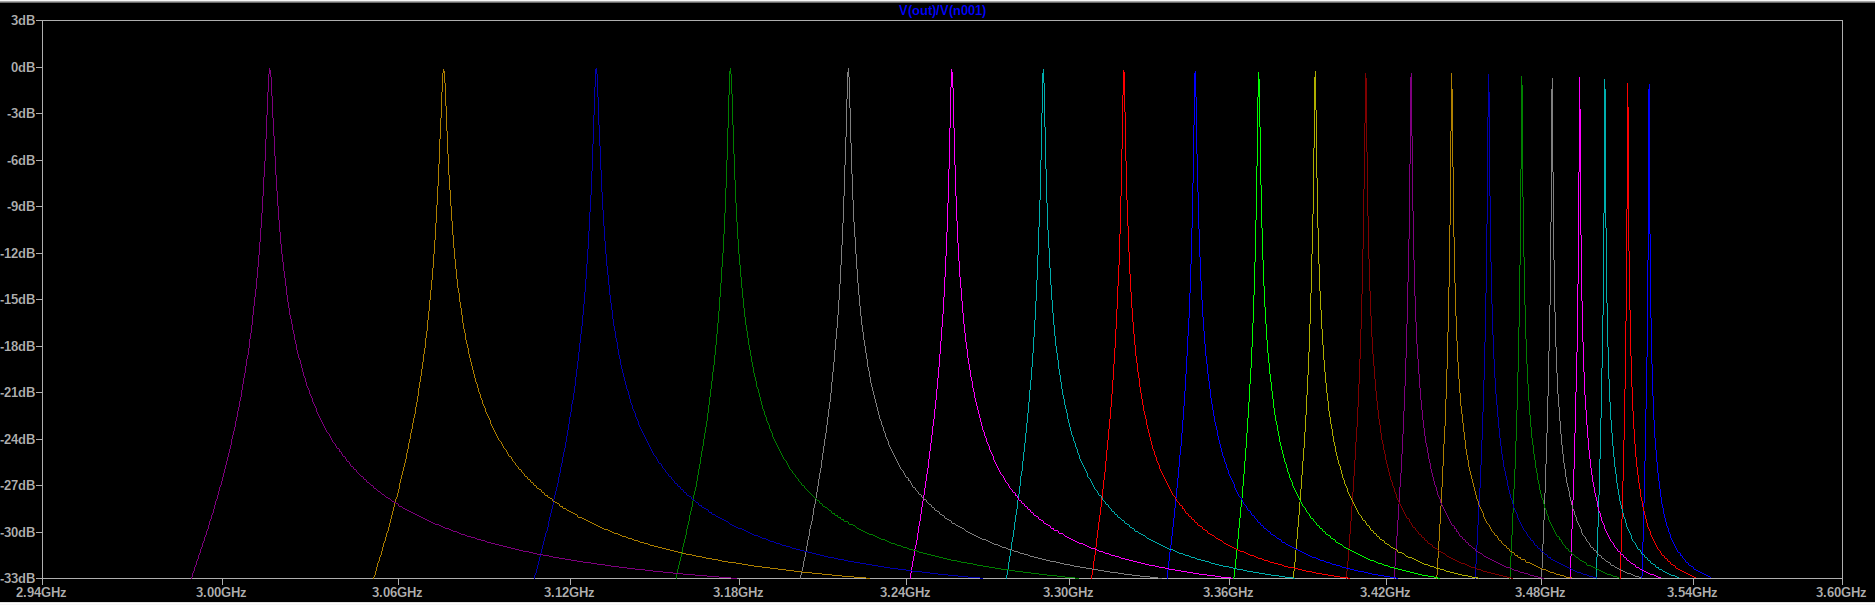
\includegraphics[width=0.8\linewidth]{exercise 6/graph_7_highqq.png}
\caption{Transfer function with $Q\approx11*10^{4}$}
\label{fig:graph_higherQ}
\end{figure}